% Options for packages loaded elsewhere
\PassOptionsToPackage{unicode}{hyperref}
\PassOptionsToPackage{hyphens}{url}
%
\documentclass[
]{article}
\usepackage{amsmath,amssymb}
\usepackage{lmodern}
\usepackage{iftex}
\ifPDFTeX
  \usepackage[T1]{fontenc}
  \usepackage[utf8]{inputenc}
  \usepackage{textcomp} % provide euro and other symbols
\else % if luatex or xetex
  \usepackage{unicode-math}
  \defaultfontfeatures{Scale=MatchLowercase}
  \defaultfontfeatures[\rmfamily]{Ligatures=TeX,Scale=1}
\fi
% Use upquote if available, for straight quotes in verbatim environments
\IfFileExists{upquote.sty}{\usepackage{upquote}}{}
\IfFileExists{microtype.sty}{% use microtype if available
  \usepackage[]{microtype}
  \UseMicrotypeSet[protrusion]{basicmath} % disable protrusion for tt fonts
}{}
\makeatletter
\@ifundefined{KOMAClassName}{% if non-KOMA class
  \IfFileExists{parskip.sty}{%
    \usepackage{parskip}
  }{% else
    \setlength{\parindent}{0pt}
    \setlength{\parskip}{6pt plus 2pt minus 1pt}}
}{% if KOMA class
  \KOMAoptions{parskip=half}}
\makeatother
\usepackage{xcolor}
\IfFileExists{xurl.sty}{\usepackage{xurl}}{} % add URL line breaks if available
\IfFileExists{bookmark.sty}{\usepackage{bookmark}}{\usepackage{hyperref}}
\hypersetup{
  hidelinks,
  pdfcreator={LaTeX via pandoc}}
\urlstyle{same} % disable monospaced font for URLs
\usepackage{graphicx}
\makeatletter
\def\maxwidth{\ifdim\Gin@nat@width>\linewidth\linewidth\else\Gin@nat@width\fi}
\def\maxheight{\ifdim\Gin@nat@height>\textheight\textheight\else\Gin@nat@height\fi}
\makeatother
% Scale images if necessary, so that they will not overflow the page
% margins by default, and it is still possible to overwrite the defaults
% using explicit options in \includegraphics[width, height, ...]{}
\setkeys{Gin}{width=\maxwidth,height=\maxheight,keepaspectratio}
% Set default figure placement to htbp
\makeatletter
\def\fps@figure{htbp}
\makeatother
\setlength{\emergencystretch}{3em} % prevent overfull lines
\providecommand{\tightlist}{%
  \setlength{\itemsep}{0pt}\setlength{\parskip}{0pt}}
\setcounter{secnumdepth}{-\maxdimen} % remove section numbering
\ifLuaTeX
  \usepackage{selnolig}  % disable illegal ligatures
\fi

\author{}
\date{}

\begin{document}

\hypertarget{problem-analysis-1}{%
\section{\texorpdfstring{Problem analysis 1
}{Problem analysis 1 }}\label{problem-analysis-1}}

The resistance of normal inhalation is divided into two parts, elastic
resistance accounts for \(70%
\) and \(30%
\) is inelastic resistance. The airway resistance concerned in the
question is inelastic resistance, accounting for \(80%
\). According to the different causes of resistance, it is divided into
the following two types. The contribution is given in square brackets:

\begin{enumerate}
\def\labelenumi{\arabic{enumi}.}
\item
  Tissue resistance \(10%
  \)
\item
  Airway resistance \(90%
  \)
\end{enumerate}

Gas molecules and the resistance between gas molecules and the tube wall
account for \(80\% ·\sim 90\%%
\). For the simplicity of problem research, and organizational
resistance contributes little to the final resistance. Therefore, only
the airway resistance is considered in the inelastic resistance section,
and the tissue resistance is not considered. Although the linear model
is easy to solve, it cannot describe the behavioral characteristics of
the complex respiratory system. The form of air flow in the respiratory
tract is very complicated and cannot be analyzed and calculated with the
simplest laminar flow.

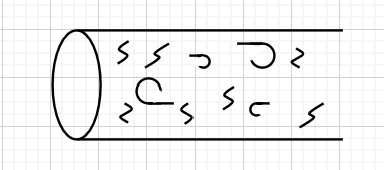
\includegraphics{C:/Users/yunswj/Desktop/mathmodel.assets/image-20211206183820998.png}

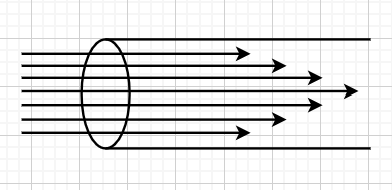
\includegraphics{C:/Users/yunswj/Desktop/mathmodel.assets/image-20211206183832213. png}

\hypertarget{model-assumptions}{%
\subsection{\texorpdfstring{Model assumptions:
}{Model assumptions: }}\label{model-assumptions}}

\begin{enumerate}
\def\labelenumi{\arabic{enumi}.}
\item
  The upper edge of the airway is a rigid round tube.
\item
  The bronchial tree is a tree-like structure \\
  with the diameter of the airway gradually decreasing from top to
  bottom. 3. According to the anatomical results, the bronchial tree is
  classified as \(23\).
\item
  The large air duct should not be deformed.
\item
  The cross-sectional radius of the small air ducts are all less than
  \(2mm\), and the internal air flow is laminar.
\item
  Physiological data of healthy men, \(K _1 = 0.34 cm ~ H _2O*S/L\),
  \(K _2 = 0.46 cm ~ H _2O*S/L\)
\item
  The relative pressure value of the outlet boundary in the CFD
  calculation is \(0\).
\item
  The calculation uses the unit system of \(cm, g, s\).
\item
  This article studies the influence of the three-dimensional
  bifurcation and bending of the bronchial channel on the flow. When the
  geometric model is generated, a smooth cylinder is used to represent
  it.
\end{enumerate}

\hypertarget{modeling}{%
\subsection{\texorpdfstring{Modeling }{Modeling }}\label{modeling}}

According to the anatomical structure of the trachea, the entire airway
is divided into three levels-the large airway with cartilage support,
the trapped airway without cartilage support, and the small airway.

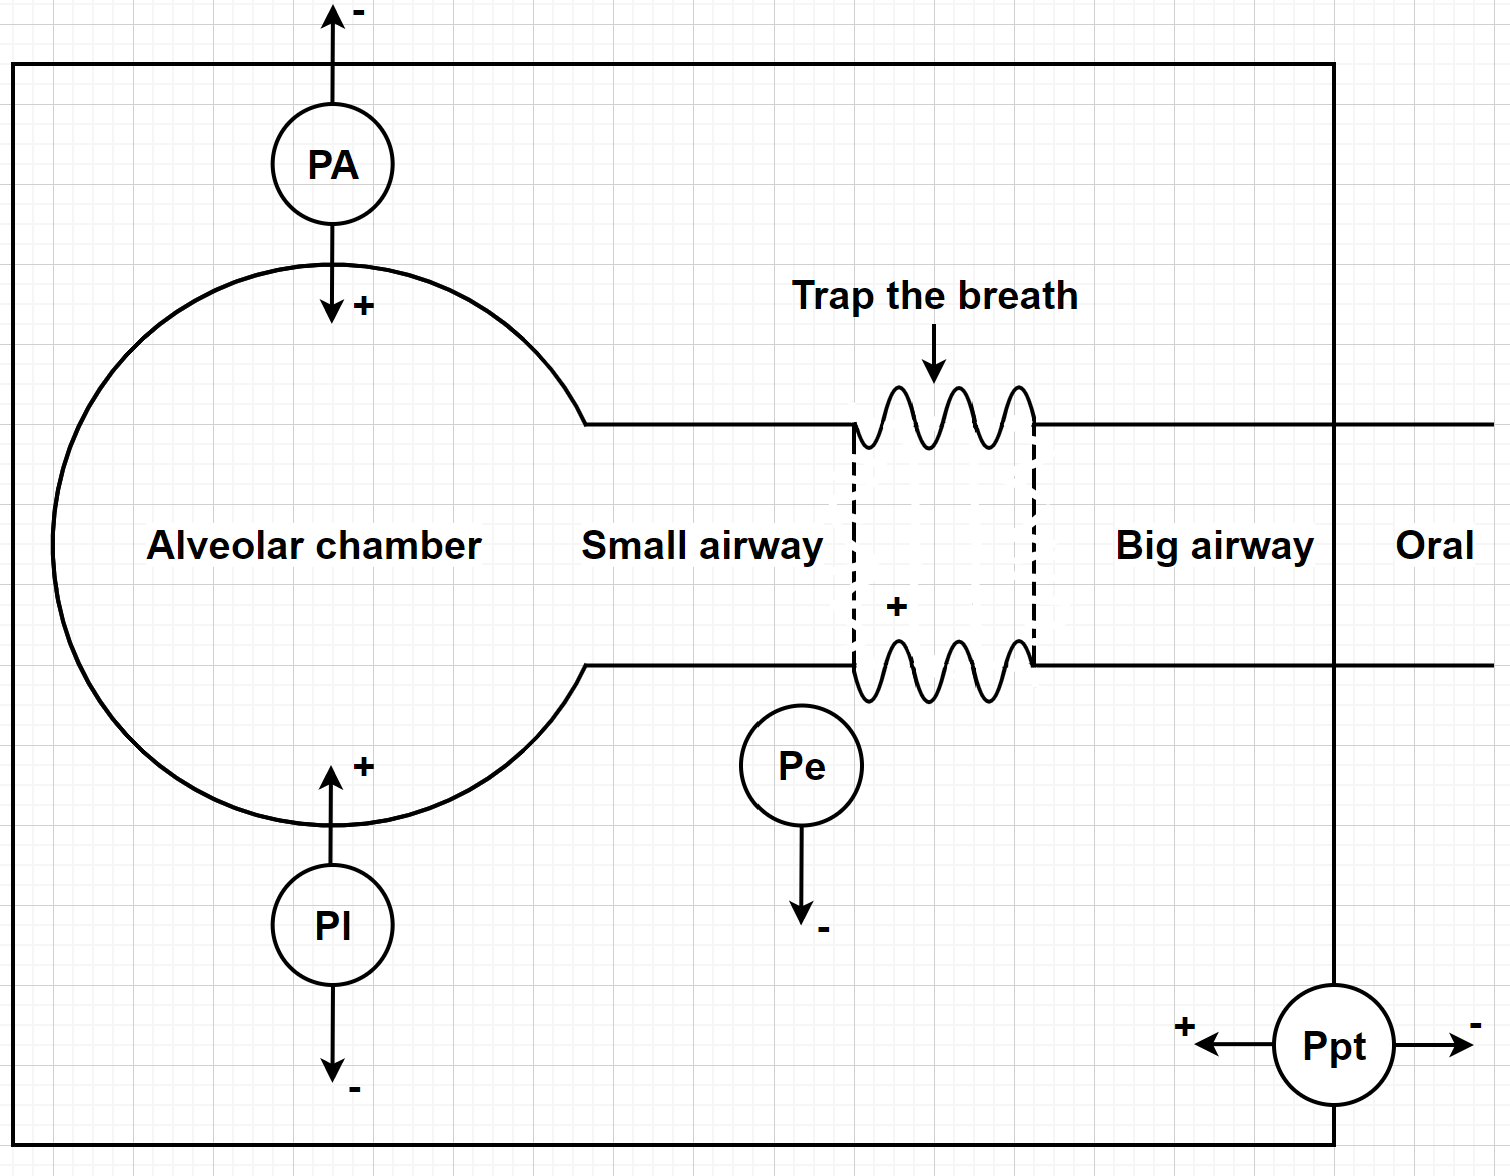
\includegraphics{C:/Users/yunswj/Desktop/mathmodel.assets/image-20211206183747794.png}

\hypertarget{1-upper-airway-rohrer-form-air-flow-resistance-described}{%
\subsubsection{\texorpdfstring{1. Upper airway Rohrer form air flow
resistance described
}{1. Upper airway Rohrer form air flow resistance described }}\label{1-upper-airway-rohrer-form-air-flow-resistance-described}}

according to the assumption of cartilage airway tube is rigid, then the
use of the form described \$ \$ Rohrer airflow resistance, in other
words the mechanical properties of the upper airway during respiration
is easily deformed large diameter airways. The expression of airway
resistance is:

\[P=R _1 \times Q +R _2 \times Q|Q|\]

where \(K _1\) and \(K _2\) are constants, which are related to the
geometric dimensions of the airway and the gas viscosity , The gas
density is related.

\hypertarget{2-trapped-airway}{%
\paragraph{\texorpdfstring{2. Trapped airway
}{2. Trapped airway }}\label{2-trapped-airway}}

Part of the airway does not contain cartilage. When the transmural
pressure on the outside is close to 0, the cross-sectional area is
reduced, which is prone to airway trapping. This part of the airway with
elasticity is called trapped airway. The internal resistance is composed
of airflow resistance and elastic resistance, and the expression of the
two functions is related to the air content in the lungs. Their diameter
expands and contracts with the change of transmural pressure, but the
length change is not obvious. Therefore, these air passages are assumed
to be a fixed-length elastic cylindrical pipe whose volume \((V _c)\)
changes with its trans-wall pressure \((P _c)\). Airway elasticity is:

\[P _c=b-{\frac{1}{a}}ln(\frac{V _cmax}{V _c}-0.999)\]

where a and b are constants. According to the \(P _c-V _c\) curve
fitting of the airway, we get \(a = 0.35cm H _2O ^{-1}\),
\(b=2cm H _2O\). The air resistance of trapped airway \((R _c)\) is as
follows:

\[R _c = K _3(\frac{V _cmax}{V _c}) ^2\]

where \(K _3\) is a constant representing \(V When _c\) reaches the
maximum value \(V _cmax\), the air resistance of the trapped airway is
trapped. \(K _3\) \(V _cmax\) \(0.21 _{cm}~H_2O*S/L,0.15L\)

\hypertarget{3-small-airway}{%
\paragraph{\texorpdfstring{3. Small airway
}{3. Small airway }}\label{3-small-airway}}

The 16 to 23 segments of the bronchus in the lungs are all called small
airways with a small cross-sectional area, so the internal airflow is
almost as laminar. The air resistance of the small airway (R \_s)
changes exponentially with the volume of air in the lung (V \_A):

\[R _s=B _s + A _s \times \exp(\frac{K _s(V _A-RV)}{VC })\]

. Among them, \(K _s, B _s, A _s, VC, RV\) are all constants, \(VC\)
represents vital capacity, and \(RV\) represents residual air volume in
the lungs. According to the change curve of \(R _s\) with \(V _A\) given
in the literature,
\(A _s = 10 cm H _2 o*S /L, B _s = 0.2cm~ H _2*S/L,K _s = -10\)
According to the physiological data of healthy men, \(VC\) and \(RV\)
take the value of \(3.95 L\) and \(1.24 L\).

\textless img
src="C:\textbackslash Users\textbackslash yunswj\textbackslash Desktop\textbackslash mathmodel.assets\textbackslash image-
20211206183903240.png "Alt =" Image-20211206183903240 "style =" Zoom: 33
is\%; "/\textgreater{}

\hypertarget{model-solution}{%
\subsection{\texorpdfstring{model solution
}{model solution }}\label{model-solution}}

is introduced in particular aspects the CFD solver, using the Fluent
solved. \(Fluent\) is calculated using the finite volume method based on
unstructured grids. After experiments, when the grid unit is
\(0.18 0.15 0.12cm\), the velocity profile at the entrance \(a\) and the
exit \(b\) have been compared near. The difference is no longer
distinguishable at the entrance. Considering that when the cell size is
\(0.12cm\), the number of cells is twice as large as that of \(0.15\),
which will increase the amount of calculation. The final grid size of
the selected cell is \( 0.15cm \) .

\hypertarget{1-solve-basic-equations}{%
\subsubsection{\texorpdfstring{(1). Solve basic equations
}{(1). Solve basic equations }}\label{1-solve-basic-equations}}

For the flow field requirements in the question, use the continuous
equation of conservation of mass and the momentum equation of
conservation of momentum. When judging the gas flow state in the tube,
it is distinguished by the size of the Reynolds number. The diameter of
the main pipe is \(1.8cm\), when the maximum inlet speed is \(150cm/s\),
the outlet pressure is 0, the gas density is \(0.001225g/cm^2\), and the
gas viscosity coefficient is \(0.0001789g/cm/s\). At this time:

\[R _E = \frac{\rho v D}{\mu}=0.001225 \times 150 \times 1.80 /0.00017894 = 1848.38\]

The Reynolds number in the main pipe is close to the critical value of
turbulence. Consider that the flow in the tube may develop into
turbulence at some moments.\\
For the flow field requirements in the question, use the continuous
equation of conservation of mass and the momentum equation of
conservation of momentum. When judging the gas flow state in the tube,
it is distinguished by the size of the Reynolds number. The diameter of
the main pipe is \(1.8cm\), when the maximum inlet speed is \(150cm/s\),
the outlet pressure is 0, the gas density is \(0.001225g/cm ^2\), and
the gas viscosity coefficient is 0.0001789g/cm/s. At this time:
\(R _E = \frac{\rho v D}{\mu}=0.001225 \times 150 \times 1.80 /0.00017894 = 1848.38\)
The Reynolds number in the main pipe is close to the critical value of
turbulence. Consider that the flow in the tube may develop into
turbulence at some moments.\\
For the flow field requirements in the question, use the continuous
equation of conservation of mass and the momentum equation of
conservation of momentum. When judging the gas flow state in the tube,
it is distinguished by the size of the Reynolds number. The diameter of
the main pipe is \(1.8cm\), when the maximum inlet speed is \(150cm/s\),
the outlet pressure is \(0\), the gas density is \(0.001225g/cm ^3\),
and the gas viscosity coefficient is\(0.0001789g/cm/s\).\\
At this time:

\[R _E = \frac{\rho v D}{\mu}=0.001225 \times 150 \times 1.80 /0.00017894 = 1848.38\]

The Reynolds number in the main pipe is close to the critical value of
turbulence. Consider that the flow in the tube may develop into
turbulence at some moments.

\hypertarget{2-selection-of-turbulence-model-equations}{%
\subsubsection{\texorpdfstring{(2). Selection of turbulence model
equations
}{(2). Selection of turbulence model equations }}\label{2-selection-of-turbulence-model-equations}}

Use the \(Spalart-Almaras\) turbulence model.

\[\frac{\partial}{\partial _t}(\rho \bar{v}) + \frac{\partial}{\partial _x{_i}}(\rho \bar{V} u _x{_i} )=\frac{1}{\sigma _{\bar{v}}}\{{\frac{\partial}{\partial _X{_j}}}[(\mu + \rho \bar{v}) ]+\rho C_b{_2}(\frac{\partial \bar{u}}{\partial x _j})\}+G _v + Y _v\]

This equation is the transfer equation of the viscosity coefficient,
where: \(\rho\) is the density, \(u _i\) is the turbulent motion
viscosity coefficient, \(\sigma, C\) are the constant coefficients.
\(G _u\) represents the generating term of the turbulent viscosity
coefficient, and \(Y _u\) represents the wall obstruction to weaken the
turbulent viscosity coefficient. The expressions are respectively:

\[G _v = \rho \bar{S} \bar{ V} C {_b{_1}}\]

\(\bar{S}\) combines the effects of vorticity and strain tensor on the
turbulent viscosity coefficient.

\[Y _u = \rho(\frac{\bar{v}}{d})^2f _ \omega C \omega _1\]

Turbulent dynamic viscosity coefficient \(\mu _1\) is
\((\mu _1 = \ rho \bar{v}f{_v{_1}})\) where

\[f _v{_1} = \frac{x ^3}{x ^3 + C^3}\]

\[\mu _1 = \rho \bar {v}[\frac{(\frac{\bar{v}}{v})^3}{(\frac{\bar{v}}{v})^3+C ^3}]\]

above In the formula, \(C _b{_1},C _b{_2},,C _v{_1},k\) are all
constants, and their value is:

\[C _b{_1}=0.1335\\

C _b{_2}=0.622\\

C _v{_1}=7.1\\C _\omega{_1}=\frac{C _b}{K ^2}+\frac{(1+C _b{_2})}{\sigma \bar{v}}\\

C _\omega{_2}=0.3\\

C _\omega{_3}=2.0,k=0.4187$\]

\hypertarget{-3-boundary-condition-constraints}{%
\subsubsection{\texorpdfstring{(. 3) boundary condition constraints.
}{(. 3) boundary condition constraints. }}\label{-3-boundary-condition-constraints}}

The physiologic data, to the averaging unit inlet velocity boundary
condition - steady calculation; Or give the change function of the
average velocity of the cross section in a breathing cycle-unsteady
calculation.

Outlet boundary: given relative pressure value. In this paper, steady
and unsteady are the same, taking \(0\). \\
Solid wall boundary: no-slip boundary condition, flow velocity is taken
as \(0\).

\hypertarget{4-constant-factor-setting}{%
\paragraph{\texorpdfstring{(4) Constant factor setting
}{(4) Constant factor setting }}\label{4-constant-factor-setting}}

\(Air Density\): \(0.001225\).

\(Viscosity\): \(0.00017894\).

Relaxation factor: \(Pressure\) 0.3,

\(Density\) is 1,

\(Body forces\) is 1,

\(Momenturn\) is \(0.7\),

\(modified turbulenced\) is \(0.8\), and

\(Turbulent viscosity\) is \(1\); in discretization, pressure is
standard discrete, and pressure-velocity coupling is discrete using the
\(SIMPLE\) method. \(Momenturn\) and \(Modified turbulent\) and
\(viscosity\) are first-order advantages.

\hypertarget{calculation-results-and-analysis}{%
\subsection{\texorpdfstring{Calculation results and analysis:
}{Calculation results and analysis: }}\label{calculation-results-and-analysis}}

Use Fluent to calculate the gas flow field calculations in the following
situations:

\begin{enumerate}
\def\labelenumi{\arabic{enumi}.}
\item
  The flow field in the tracheal tree that is directly connected to the
  bifurcated four to four levels and is completely transitioned.
\item
  The unsteady calculation of the flow field in the tracheal tree with
  the transition of the complete tube end smoothly and bifurcated to
  three levels.
\item
  The unsteady calculation of the flow field in the tracheal tree that
  is smoothly bifurcated to the fourth stage, and compares the effect of
  the bifurcation series on the gas flow in the previous stages.
\end{enumerate}

In order to facilitate the establishment of the model, here we can
choose the plane view of several parts of the airway cross-section. As
shown, \(F1\) represents the cross-section when the coordinates of \(Z\)
are \(0\). \(F2\) is the corresponding section when the coordinate of
\(X\) is \(0\), corresponding to the section on the front and back walls
of the trachea. Now we have inserted the left bronchus with four
cross-sections \(L1, L2, L3, L4\), and the right main bronchus with
three cross-sections \(R1, R2, R3\).

\begin{figure}
\centering
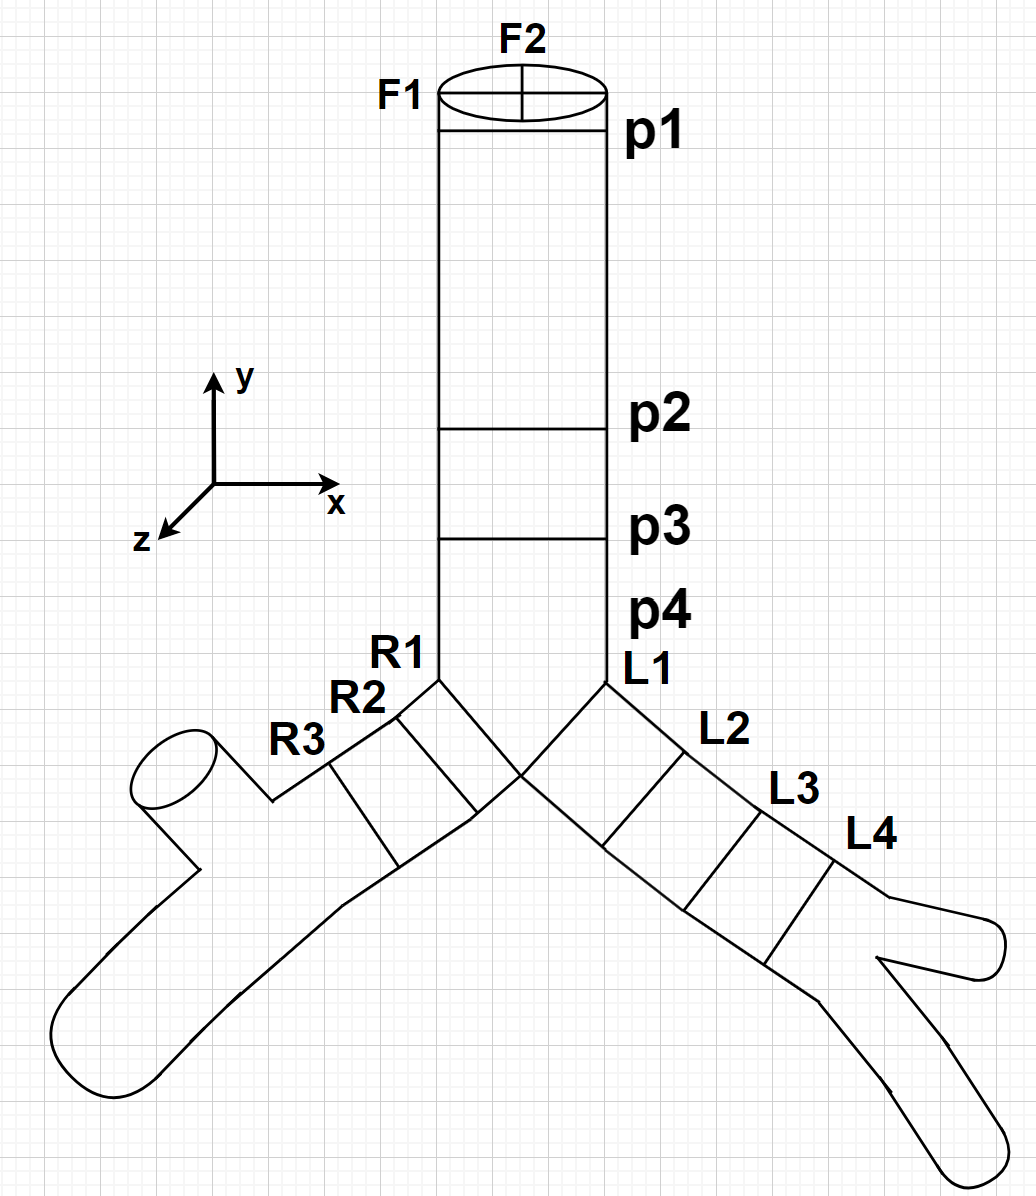
\includegraphics{C:/Users/yunswj/Desktop/mathmodel.assets/image-20211206183708516.png}
\caption{image-20211206183708516}
\end{figure}

In order to simplify the model and facilitate the actual operation, here
we adopted the direct connection model establishment method of
cylindrical pipes for the pipe connection at the bifurcation. We modeled
from the entrance of the main trachea to the fourth-level lung bronchus,
using a tetrahedral mesh to automatically divide it.\\
Under normal circumstances, since the human body's ventilation volume
per minute is at least \(3 L/min\) (deep anesthesia), it can exceed
\(100 L/min\) (during exercise), and more than \(200 L/min\) (measured
maximum) in a short period of time. Breath volume). Based on the current
medical research and the rationality of the experiment, we select the
diameter of the main bronchus at the entrance of healthy lungs of adults
is \(1.8 cm\), and the average import speed is \(50\sim1666 cm/s\). In
the resting state, the breath is \(12\sim18\) times per minute, and the
import speed is \(150cm/s\). In order to obtain the results that can
converge quickly, we use the \(Spalart-Allmaras\) turbulence model to
solve the problem, and iterate a total of \(58\) steps.

Through the analysis of the air velocity distribution in the lungs, it
can be known that because the angle between the right bronchus and the
main bronchus is smaller, the air flow in the right lung is greater than
that in the left lung. Based on the average inlet velocity of
\(150 cm/s\), the maximum velocity in the main flow field has reached
\(180 cm/s\), and the Reynolds number calculated from the maximum
velocity of the main flow field is \(2200\), which is very close. The
critical value for turbulent flow is \(2300\). The local velocity in the
trachea of the right bronchus reached a maximum of \(220 cm/s\).

Through researching relevant data, it is found that when the connection
is directly connected by a cylindrical tube, due to the large angle
between the left bronchus and the main trachea, the gas is shunted after
passing through the main trachea during inhalation, and there is a
longer section of the trachea after the shunt. The phenomenon of air
flow separation occurred in the obvious stagnation zone. This situation
is not conducive to the flow and transmission of gas in the human
trachea. However, in the transitional connection model of the curved
pipe, a pair of vortices with opposite rotation directions appear in the
secondary flow. In the model of the straight pipe connection, the
velocity distribution on the secondary flow is not so obvious.

The unsteady calculation of the three-stage bifurcated pipe model of the
elbow transition \\
is to study the gas flow state in the bronchus during a breathing cycle.
\\
Boundary conditions\\
We use a tetrahedral grid with a unit height of \(0.15cm\). A normal
person breathes \(12~18\) times per minute in a calm state, and an
average of \(15\) times is used in the calculation, so a cycle is
determined to be \(4.0s\), and the human breathing frequency is
\(0.25Hz\) at this time. The maximum speed of the import is
\(150 cm/s\). According to the existing physiological research data, the
relationship of import speed with time is

\[v=150 \times \sin(2 \times \pi \times t/T)\]

where \(T=4 s\). Other boundary conditions are the same as before.

\#问题二

\hypertarget{analysis-of}{%
\subsection{\texorpdfstring{Analysis of
}{Analysis of }}\label{analysis-of}}

the second question On the basis of the fluid model of the first
question, consider the gas flow in the bronchus when there is a mass
with a radius of 0.7cm at the bifurcation. Assume that a spherical
foreign body with a diameter of \(0.7cm\) grows at the bifurcation of
the left and right bronchus at the end of the normal main bronchus. Then
use \(Fluent\) for modeling calculations.

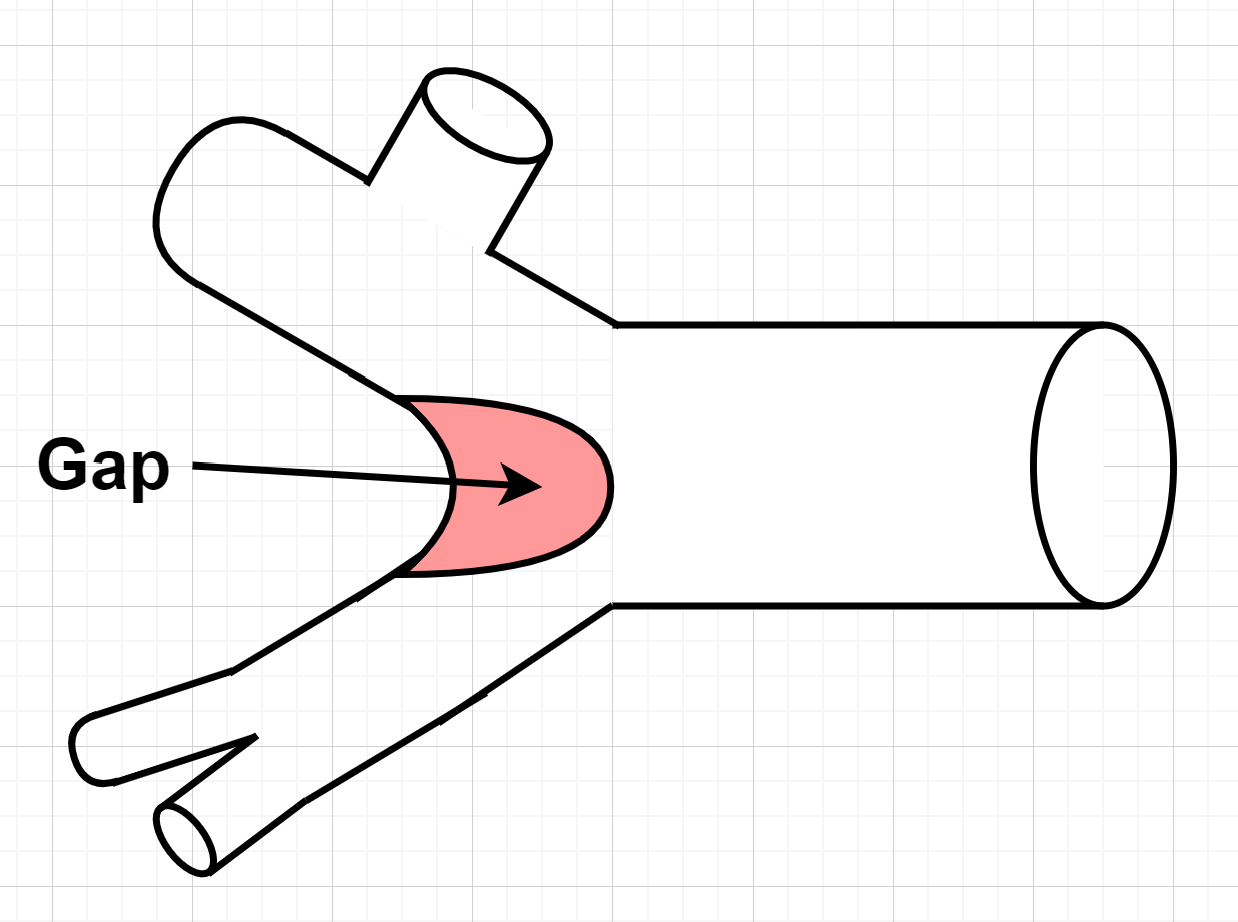
\includegraphics{C:/Users/yunswj/Desktop/mathmodel.assets/image-20211206190906904.png}

\hypertarget{the-calculation}{%
\subsection{\texorpdfstring{The calculation
}{The calculation }}\label{the-calculation}}

uses tetrahedral unit division Grid, the unit height is \(0.15 cm\), and
the total number of grids is \(106602\). The setting of the boundary
conditions is the same as that of the three-stage bifurcated pipe. When
performing unsteady calculations, the breathing period is 4 seconds, the
iteration time step is \(0.05s\), and the total number of iterations is
\(80\) times. After calculation, the air velocity is up to \(238cm/s\).

\hypertarget{result-analysis}{%
\subsection{Result analysis}\label{result-analysis}}

When the maximum inhalation flow occurs in one second, the study of the
F1 cross-section shows that in the abnormal situation, because the
pipeline suddenly becomes smaller, high-speed fluid areas appear on both
sides of the branch pipe. When the speed of the intake pipe is the same,
the flow velocity in the normal bronchial main pipe is slightly larger
than the gas flow velocity in the bronchus causing the disease. At a
position far away from the lesion, the velocity profile of the two is
similar, but at the location of the lesion. Attachment, the flow pattern
has changed a lot. It is concluded that the narrowing of the bronchial
tubes on both sides caused by the lesions increases the velocity in this
part. The location of the lesion is on the inner side of the trachea.
After branching from the main pipe, the speed of the secondary flow
deviates to the outer side of the tube wall, so that the shearing force
on the outer side wall of the bronchus is greater than the inner side of
the tube wall. After a period of development in the sub-pipe. The flow
situation far away from the damage is the same as before.

\hypertarget{question-three}{%
\section{\texorpdfstring{Question three
}{Question three }}\label{question-three}}

varying the frequency and intensity of breathing, the case of
intratracheal Discussion winter tree

Abstract: The gas barrier one or several non-linear element does not
describe the whole breathing pipe for conventional mechanical model - a
bronchial tree drawbacks. Based on the anatomical structure of the
bronchial tree of the lungs, this paper uses the Golden three-level
airway model as a blueprint to establish a multi-chamber, non-linear
airway grading intensive parameter model of respiratory mechanics, and
draws that the resistance of the trachea to the airway resistance of 16
to 23 levels The contribution of is the largest, and it is equal to the
4th power of the tracheal cross-sectional radius. The corresponding
pulmonary bronchial tree spatial asymmetric model was established, and
the computational fluid dynamics software Fluent was used for numerical
solution. The effect of different bending modes at the bifurcation of
the trachea and the influence of different meshes on the calculation
results were purposefully compared. . By establishing a trigeminal
tracheal tree lesion model, the increase in airflow velocity at the gap
is obtained

\end{document}
